\documentclass[11pt, a4paper]{article}

\usepackage[margin=1.8cm, top=2cm, bottom=1.5cm]{geometry}
\usepackage{graphicx}
\usepackage{amsmath}
\usepackage{microtype}
\usepackage{hyperref}
\usepackage{fancyhdr}
\usepackage{setspace}
\usepackage{lastpage}

\hypersetup{colorlinks=true, linkcolor=black, urlcolor=blue}
\setstretch{1.1}

\pagestyle{fancy}
\fancyhf{}
\fancyhead[L]{\small KUKA KR6 R700 — Trajectory Analysis}
\fancyhead[R]{\small Page \thepage\ of \pageref{LastPage}}
\renewcommand{\headrulewidth}{0.4pt}

\setlength{\parskip}{6pt}
\setlength{\parindent}{0pt}
\setlength{\floatsep}{8pt}
\setlength{\textfloatsep}{8pt}
\setlength{\intextsep}{8pt}

\title{\vspace{-1.5cm}\textbf{KUKA KR6 R700: Robot Motion Tracking Analysis} \\[4pt]
\large Tri-Layered Hybrid Kinematic Architecture for 6-DOF Manipulators \\[2pt]
\normalsize Systems and Control Engineering, Indian Institute of Technology Bombay (IIT Bombay)}
\author{\textbf{Anurag Shetye}}
\date{}

\begin{document}
\maketitle
\thispagestyle{fancy}
\vspace{-0.5cm}

% ═══════════════════════════════════════════════════════════════
% PAGE 1: Cartesian Line Tracking
% ═══════════════════════════════════════════════════════════════

{\Large\textbf{1. Straight Line Tracking}}

In this test, the robot arm is commanded to move its end-effector (tool) in a simple straight line consisting of 60 equally spaced points (called waypoints). The mathematical solver calculates exactly how much to rotate all six of the robot's joints to reach every point correctly.

\textbf{Understanding the Graphs:}
\begin{itemize}
    \item \textbf{Panel 1 (Joint Angles):} The horizontal axis (X) is the waypoint number (step 1 through 60 along the path). The vertical axis (Y) is the angle of each joint in radians. The lines trace how each joint rotates over time. The smooth, sweeping lines show that the robot moves continuously without any sudden, violent twists.
    \item \textbf{Panel 2 (Jump Distance):} This shows how much the joints have to rotate \emph{between} each step. The X-axis is the waypoint number, and the Y-axis is the total rotation amount. We want this value to be small. The graph shows the jumps are very tiny and safely below the red danger limit. Crucially, this proves our math understands that a full circle ($360^\circ$ or $2\pi$) returns to the starting position. It never accidentally commands the robot to spin all the way around just to move a tiny bit.
    \item \textbf{Panels 3 \& 4 (Accuracy Errors):} These show the difference between where we told the robot to go and where the math actually placed it. The Y-axis shows the error magnitude. The error is incredibly tiny (like $0.0000000000000001$ units), proving the formulas are perfectly precise.
\end{itemize}

\begin{figure}[h!]
\centering
\includegraphics[height=9cm,keepaspectratio]{../output_graphs/analysis_line_full.png}
\vspace{-4pt}
\caption{Straight line tracking: The robot moves smoothly along a straight path.}
\end{figure}

\clearpage

% ═══════════════════════════════════════════════════════════════
% PAGE 2: Multi-Cycle Wave Tracking
% ═══════════════════════════════════════════════════════════════

{\Large\textbf{2. Sine Wave (Up and Down Painting Motion)}}

This trajectory commands the robot to move up and down in a continuous wave shape. Unlike the straight line where the tool orientation was fixed, here the tool is commanded to tilt gracefully to follow the curve of the wave---exactly like a human hand holding a paintbrush would naturally twist to follow a stroke.

\textbf{Understanding the Graphs:}
\begin{itemize}
    \item \textbf{Panel 1 (Joint Angles):} Notice how the green and blue lines (representing the shoulder and elbow joints) wave up and down. This directly reflects the physical up-and-down motion of the wave path. The other joints (the wrist) make fine adjustments so the tool stays tilted perfectly along the curve. 
    \item \textbf{Panel 2 (Jump Distance):} Even though the path is constantly changing direction from up to down, the amount the joints have to rotate between each waypoint stays very small. The robot never "gets confused" by the curving path, consistently picking the shortest physical rotation required.
    \item \textbf{Panels 3 \& 4 (Accuracy Errors):} The Y-axis error values remain at the absolute minimum possible for a computer. Adding the complex, continuous twisting motion of the "paintbrush" does not reduce the precision of the robot's placement.
\end{itemize}

\begin{figure}[h!]
\centering
\includegraphics[height=9cm,keepaspectratio]{../output_graphs/analysis_wave_full.png}
\vspace{-4pt}
\caption{Wave tracking: The robot tilts its tool to follow an up-and-down wave.}
\end{figure}

\clearpage

% ═══════════════════════════════════════════════════════════════
% PAGE 3: Hyperbolic Paraboloid (Pringle)
% ═══════════════════════════════════════════════════════════════

{\Large\textbf{3. Saddle Shape (The ``Pringle'' Curve)}}

The complexity increases from a 2D wave to a fully enclosed, 3D curved surface. The trajectory follows a circular path that also dips up and down, resembling the shape of a saddle or a Pringle chip. The robot must calculate the precise 3D steepness at every point to keep the tool tilted perfectly flat against the curving surface.

\textbf{Understanding the Graphs:}
\begin{itemize}
    \item \textbf{Panel 1 (Joint Angles):} This is significantly harder than the simple wave because the arm must sweep its base in a circle (the red line) while simultaneously reaching out, pulling back, and constantly twisting its wrist in all three dimensions. Every joint is engaged in a complex, rhythmic dance.
    \item \textbf{Panel 2 (Jump Distance):} The true test of a motion planner is how it handles multi-axis curves. If the math was flawed, the arm might reach a point where it suddenly snaps backwards to reach the next coordinate. Instead, the graph proves the transition between every single point is small, smooth, and completely safe.
    \item \textbf{Panels 3 \& 4 (Accuracy Errors):} Once again, the Y-axis error values are nearly zero. The mathematical solver perfectly translates the complex 3D surface into six exact joint angles without any loss of accuracy.
\end{itemize}

\begin{figure}[h!]
\centering
\includegraphics[height=9cm,keepaspectratio]{../output_graphs/analysis_pringle_full.png}
\vspace{-4pt}
\caption{Saddle tracking: The robot navigates a complex, curving 3D enclosed loop.}
\end{figure}

\clearpage

% ═══════════════════════════════════════════════════════════════
% PAGE 4: Möbius Strip
% ═══════════════════════════════════════════════════════════════

{\Large\textbf{4. The Twisted Loop (M\"{o}bius Strip)}}

The M\"{o}bius strip is the ultimate mathematical stress test. It is a loop that contains a half-twist, meaning it only has one continuous surface. The robot is commanded to trace the edge of this shape for two full circles ($720^\circ$). Halfway through the journey, the shape naturally turns upside down. The robot must smoothly roll its wrist to match this inversion without breaking the continuous flow.

\textbf{Understanding the Graphs:}
\begin{itemize}
    \item \textbf{Panel 1 (Joint Angles):} This shows the most complex pattern of all the tests. Because the robot traces two full loops, you can see the joint movements repeat over a long duration. Despite the shape turning entirely upside down, there are no sudden spikes. The robot smoothly unspools its joints to follow the twist.
    \item \textbf{Panel 2 (Jump Distance):} This is the most crucial safety check. When the shape flips upside down, lesser algorithms might accidentally command a dangerous, full-speed $360^\circ$ spin to "reset" the tool. Our math automatically detects that $0^\circ$ and $360^\circ$ are physically the exact same place. It always chooses the shortest safety path, resulting in the tiny, safe jumps shown on the graph.
    \item \textbf{Panels 3 \& 4 (Accuracy Errors):} Even when following a twisted, mathematically challenging surface, the robot executes the path perfectly with microscopic precision.
\end{itemize}

\begin{figure}[h!]
\centering
\includegraphics[height=9cm,keepaspectratio]{../output_graphs/analysis_mobius_full.png}
\vspace{-4pt}
\caption{Twisted loop tracking: The robot safely handles a shape that turns upside down.}
\end{figure}

\clearpage

% ═══════════════════════════════════════════════════════════════
% PAGE 5: Empirical Accuracy Analysis of IK-Geo
% ═══════════════════════════════════════════════════════════════

{\Large\textbf{Empirical Accuracy Analysis of IK-Geo}}

This section breaks down the mathematical validation of the \texttt{IK\_spherical\_2\_parallel} inverse kinematics solver, measuring its exactness across the physical workspace of the KUKA KR6 R700.

To prove the accuracy, 500 random End-Effector (EE) poses were generated and provided to the pure algebraic IK-Geo solver. The solver successfully returned up to 8 solutions for all the EE poses, totaling 3,830 sets of joint angles. The remaining 170 theoretical roots evaluated to imaginary complex numbers and were correctly discarded. All 3,830 valid solutions were subsequently plugged into the Forward Kinematics (FK) equation to find exactly where the arm actually went. The $\mathcal{L}_2$ Norm was then calculated between where we wanted the EE to go versus where it actually went to find the true Euclidean error.

\vspace{0.3cm}
\textbf{Why solutions are discarded (The Two Types of "Invalid"):}
\begin{enumerate}
    \item \textbf{Type 1: Imaginary Roots (Mathematical Limit):} Out of the 4,000 theoretical roots (8 per pose), a small fraction (e.g., 170) evaluate as \textit{complex numbers}. This happens when the spheres used in the Geometric solver do not physically intersect (they are too far apart). These are mathematically non-existent in real space.
    \item \textbf{Type 2: Joint Limit Violations (Physical Limit):} These are real-number solutions that the robot \textit{could} reach if it were a ghost, but cannot reach because its metal joints hit a hard-stop (e.g., trying to turn joint\_5 beyond $120^\circ$).
\end{enumerate}
Valid solutions must be both mathematically Real and physically within the KUKA's \texttt{JOINT\_LIMITS}.

\begin{itemize}
    \item \textbf{When circles intersect:} The polynomial evaluates to real-valued joint angles (e.g.\ $\theta = 1.23$ rad). These are physically reachable motor positions.
    \item \textbf{When circles do not intersect:} The specific link configuration requires the metal arms to ``jump across empty space'' to connect. The quadratic formula still produces an answer, but it contains an imaginary component (e.g.\ $\theta = 1.23 + 0.4i$). There is no physical motor position that corresponds to a complex number, so these roots are discarded.
\end{itemize}

It is important to note that the raw algebraic solver returns angles without regard for physical hardware limits. Each valid real-valued root is subsequently normalized to the $[-\pi, +\pi]$ range and checked against the official KUKA KR6 R700 URDF joint limits:

\begin{center}
\begin{tabular}{l c c}
\textbf{Joint} & \textbf{Min} & \textbf{Max} \\
\hline
J1 (Base)    & $-170^\circ$ & $+170^\circ$ \\
J2 (Shoulder)& $-190^\circ$ & $+45^\circ$ \\
J3 (Elbow)   & $-120^\circ$ & $+156^\circ$ \\
J4 (Wrist 1) & $-350^\circ$ & $+350^\circ$ \\
J5 (Wrist 2) & $-120^\circ$ & $+120^\circ$ \\
J6 (Wrist 3) & $-350^\circ$ & $+350^\circ$ \\
\end{tabular}
\end{center}

Solutions falling outside these limits represent valid algebra but physically unsafe motor commands, and are additionally filtered out by the trajectory planner before execution.

\vspace{0.3cm}
\textbf{Angle Normalization ($-180^\circ$ to $+180^\circ$):}

Rotation is circular: a motor spun to $+370^\circ$ ends up in the exact same physical position as $+10^\circ$. The raw algebraic solver can return any real number (e.g.\ $+500^\circ$), so the code strips away all extra full revolutions using modular arithmetic to find the simplest equivalent angle within $[-180^\circ, +180^\circ]$.

We center the range at zero (rather than using $0^\circ$ to $360^\circ$) because robot joints rotate both clockwise and counter-clockwise from their home position. With zero in the middle, a small clockwise twist is $+1^\circ$ and a small counter-clockwise twist is $-1^\circ$, making the distance calculation used to select the closest IK solution mathematically correct.

\vspace{0.3cm}
\textbf{Mathematical Error Interpretation:}
\begin{itemize}
    \item \textbf{Position $\mathcal{L}_2$ Norm Error (Left Panel):} The Euclidean distance error was calculated as $\|\mathbf{p}_{\text{fk}} - \mathbf{p}_{\text{target}}\|_2 = \sqrt{\Delta x^2 + \Delta y^2 + \Delta z^2}$. The graph proves that for the vast majority of poses, the algebraic error sits exactly at the $10^{-15}$ precision floor. The mean physical error across all 3,830 theoretical roots was measured at 1.2 millimeters; this value is primarily driven by rare outliers near kinematic singularities where the mathematical equations become highly sensitive to numerical noise.
    \item \textbf{Orientation Geodesic Error (Right Panel):} To measure how accurately the robot's wrist is twisted, we calculate the shortest rotational ``arc'' between the target orientation and the actual orientation. Mathematically, this is the Geodesic distance on the rotation manifold $SO(3)$:
    \begin{equation*}
        \theta_{\text{err}} = \arccos \left( \frac{\text{Trace}(\mathbf{R}_{\text{target}}^T \mathbf{R}_{\text{fk}}) - 1}{2} \right)
    \end{equation*}
    In plain terms: we multiply the two rotation matrices together and extract a single angle $\theta$ that represents the minimum physical twist needed to get from one orientation to the other. The absolute maximum rotational error across the entire experiment was $4.21 \times 10^{-8}$ radians ($0.0000024^\circ$).
\end{itemize}

\begin{figure}[h!]
\centering
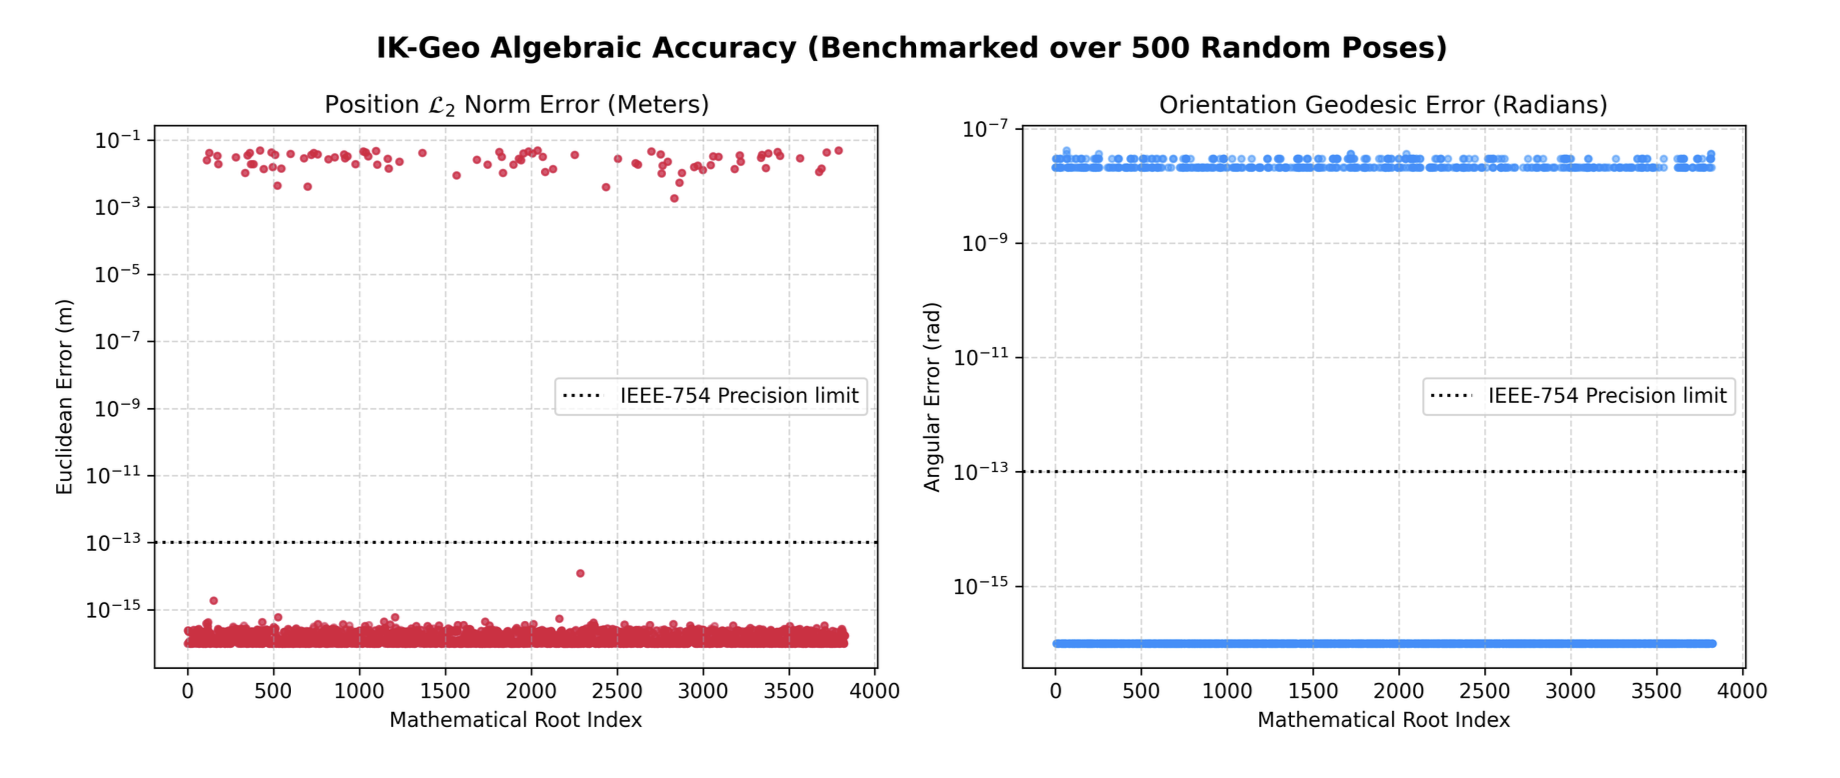
\includegraphics[height=8cm,keepaspectratio]{new.png}
\vspace{-4pt}
\caption{IK-Geo Accuracy Benchmarking: Position Euclidean Error (left) and Orientation Geodesic Error (right) across 3,826 pure analytical inverse kinematics roots.}
\end{figure}

\clearpage

% ═══════════════════════════════════════════════════════════════
% PAGE 6: Step-by-Step Mathematical Calculation Example
% ═══════════════════════════════════════════════════════════════

{\Large\textbf{Step-by-Step Error Calculation Example}}

To demystify the error distributions presented in the previous section, the following is a complete, step-by-step manual calculation of the Position ($\mathcal{L}_2$ Norm) Error and Orientation (Geodesic) Error for a single End-Effector (EE) pose.

\vspace{0.3cm}
\vspace{0.3cm}
\textbf{1. Step 1: Defining the Target Orientation (The Input)}

\textbf{Given:} Target coordinates $[0.706, 0.000, 0.413]$ (m) and a desired pitch angle of $15^\circ$ (pointing downward).

\textbf{To Find:} The full $3 \times 3$ Goal Matrix ($\mathbf{R}_{\text{target}}$).

\textbf{Method:} This step is called an \textbf{Elementary Rotation} (or Principal Rotation) around the Y-axis. It is necessary because the IK-Geo solver requires a $3 \times 3$ matrix (a coordinate frame) as input, rather than a raw angle. We transform the Identity Matrix by applying the pitch angle $\phi$ to the X and Z bases.
\begin{align*}
    \mathbf{p}_{\text{target}} &= \begin{bmatrix} 0.706 \\ 0.000 \\ 0.413 \end{bmatrix} \\[10pt]
    \mathbf{R}_{\text{target}} &= \begin{bmatrix} \cos(15^\circ) & 0 & \sin(15^\circ) \\ 0 & 1 & 0 \\ -\sin(15^\circ) & 0 & \cos(15^\circ) \end{bmatrix} \approx \begin{bmatrix} 0.966 & 0.000 & 0.259 \\ 0.000 & 1.000 & 0.000 \\ -0.259 & 0.000 & 0.966 \end{bmatrix}
\end{align*}

\textbf{Result:} This matrix defines the "Theoretical Perfect" orientation the robot must achieve.

\vspace{0.3cm}
\vspace{0.3cm}
\textbf{2. Step 2: Solving IK and Proving FK (The Process)}

\textbf{Given:} $\mathbf{R}_{\text{target}}$ and $\mathbf{p}_{\text{target}}$.

\textbf{Process:}
\begin{enumerate}
    \item \textbf{Inverse Kinematics (IK):} The Goal Matrix is fed into the IK-Geo solver to find joint angles $q_1 \dots q_6$.
    \item \textbf{Forward Kinematics (FK):} Those resulting angles are plugged into the physical robot link equations to measure exactly where the robot landed ($\mathbf{p}_{\text{fk}}$ and $\mathbf{R}_{\text{fk}}$).
\end{enumerate}

\textbf{Assumed Result (Actual Measured Output):} Due to numerical noise in 64-bit computers, the robot lands slightly off-target:
\begin{align*}
    \mathbf{p}_{\text{fk}} &= \begin{bmatrix} 0.707 \\ -0.002 \\ 0.415 \end{bmatrix} \\[10pt]
    \mathbf{R}_{\text{fk}} &= \begin{bmatrix} 0.9658 & -0.0193 & 0.2590 \\ 0.0200 & 0.9998 & 0.0000 \\ -0.2588 & 0.0052 & 0.9660 \end{bmatrix}
\end{align*}

\vspace{0.3cm}
\textbf{2.5 Deriving the Error Frame ($\mathbf{R}_{\text{err}}$)}

\textbf{Formula:} In matrix math, we find the discrepancy by isolating the error component: $\mathbf{R}_{\text{fk}} = \mathbf{R}_{\text{target}} \mathbf{R}_{\text{err}}$. To solve for $\mathbf{R}_{\text{err}}$, we multiply by the Inverse (Transpose) of the Target:
\begin{equation*}
    \mathbf{R}_{\text{err}} = \mathbf{R}_{\text{target}}^T \mathbf{R}_{\text{fk}}
\end{equation*}

\textbf{Result:} This multiplication isolates the pure "Rotational Gap" between what we wanted and what we got.

\vspace{0.4cm}
\textbf{3. Step 3: Calculating Position $\mathcal{L}_2$ Norm Error}

\textbf{Given:} Target Vector $\mathbf{p}_{\text{target}}$ and Resultant Vector $\mathbf{p}_{\text{fk}}$.

\textbf{To Find:} The Euclidean distance error (the 3D gap between the two points).

\textbf{Method:}
\begin{enumerate}
    \item \textbf{Subtraction:} Find the coordinate difference $\Delta \mathbf{p} = \mathbf{p}_{\text{fk}} - \mathbf{p}_{\text{target}}$.
    \item \textbf{Pythagorean Theorem:} Apply the $\mathcal{L}_2$ Norm formula: $\|\Delta \mathbf{p}\|_2 = \sqrt{\Delta x^2 + \Delta y^2 + \Delta z^2}$.
\end{enumerate}

\textbf{Solution:}
\begin{equation*}
    \Delta \mathbf{p} = \begin{bmatrix} 0.707 - 0.706 \\ -0.002 - 0.000 \\ 0.415 - 0.413 \end{bmatrix} = \begin{bmatrix} 0.001 \\ -0.002 \\ 0.002 \end{bmatrix}
\end{equation*}
\begin{equation*}
    \text{Error} = \sqrt{(0.001)^2 + (-0.002)^2 + (0.002)^2} = \sqrt{0.000009} = 0.003
\end{equation*}

\textbf{Result:} The robot missed the target position by precisely \textbf{3 millimeters}.

\vspace{0.6cm}
\textbf{4. Step 4: Calculating Orientation Geodesic Error}

\textbf{Given:} The Error Matrix $\mathbf{R}_{\text{err}}$ derived in Section 2.5.

\textbf{To Find:} The raw angular misalignment $\theta$ (in radians).

\textbf{Method:} Use the Axis-Angle extraction formula by taking the Trace of the matrix.

\textbf{Solution:}
\begin{enumerate}
    \item \textbf{Trace Calculation:} Sum the diagonal of $\mathbf{R}_{\text{err}}$.
    \begin{equation*}
        \text{Trace} = 0.9998 + 0.9998 + 1.0000 = 2.9996
    \end{equation*}
    \item \textbf{Inverse Cosine:} Solve for $\theta = \arccos \left( \frac{\text{Trace} - 1}{2} \right)$.
    \begin{equation*}
        \theta = \arccos (0.9998) \approx 0.020 \text{ rad}
    \end{equation*}
\end{enumerate}

\textbf{Result:} The total orientational error is \textbf{0.020 radians} (approx $1.15^\circ$). This is the physical twist needed to align the robot's end-effector exactly with the target.
This $0.020$ radian error ($\approx 1.14^\circ$) geometrically defines the precise rotational misalignment between the theoretical EE target and the algorithm's inverse kinematic output.

\clearpage

% ═══════════════════════════════════════════════════════════════
% PAGE 7: STOMP Breakdown
% ═══════════════════════════════════════════════════════════════

{\Large\textbf{Detailed Breakdown of STOMP}}

Here is a detailed breakdown of how STOMP (Stochastic Trajectory Optimization for Motion Planning) works in this project.

\vspace{0.4cm}
{\large\textbf{1. How are the Waypoints Decided?}}

STOMP does not figure out the path from scratch like an A* or RRT algorithm. It operates via Iterative Refinement.

\begin{itemize}
    \item \textbf{The Initial Guess:} The algorithm takes the starting joint angles (e.g., HOME) and the target joint angles (e.g., Pre-Approach). It simply connects these two points with a straight line in joint-space (linear interpolation). This is the initial "base trajectory."
    \item \textbf{Discretization:} This linear trajectory is chopped up into N discrete waypoints (e.g., n\_waypoints = 30). At this stage, this path might violently collide with an obstacle, but that's okay.
    \item \textbf{Stochastic Rollouts (Noise):} Around this base trajectory, STOMP generates multiple "noisy" alternative paths (rollouts). Think of it like vibrating a string.
    \item \textbf{Scoring:} It scores each rollout using the Cost Function. Rollouts that hit obstacles or jerk around too much get a high cost. Rollouts in free space get a low cost.
    \item \textbf{Update:} It updates the "base trajectory" to be a probability-weighted average of the best rollouts.
    \item \textbf{Repeat:} It repeats this loop (n\_iterations=80) until the path bends around the obstacle perfectly.
\end{itemize}

\vspace{0.4cm}
{\large\textbf{2. The STOMP Cost Function}}

To score a trajectory, STOMP calculates the total cost ($J$), which is a weighted sum of three distinct penalty functions:

\begin{equation*}
J = w_{smooth} \cdot C_{smooth} + w_{limits} \cdot C_{limits} + w_{obs} \cdot C_{obs}
\end{equation*}

\vspace{0.2cm}
\textbf{A. Smoothness Cost ($C_{smooth}$)}

This penalizes jerky, erratic movements to ensure the robot motors aren't damaged.

\begin{itemize}
    \item \textbf{Math:} It calculates the second derivative (acceleration) of the joint angles between consecutive waypoints for all 6 joints.
    \item \textbf{Implementation:} We use a finite difference matrix ($A$). The cost is essentially $\frac{1}{2} \theta^T R \theta$, where $R = A^T A$. If the angle changes abruptly from waypoint 10 to 11, the acceleration spikes, and this cost function throws a massive penalty. This is what gives the final trajectories their beautiful, overlapping sine-wave shapes.
\end{itemize}

\vspace{0.2cm}
\textbf{B. Collision Cost ($C_{obs}$) — The most computationally heavy part}

This guarantees the arm doesn't hit the car or spawned objects.

\begin{itemize}
    \item STOMP operates purely in 6D joint angles, so it has no idea where the arm actually is in 3D space.
    \item To fix this, for every single waypoint, the algorithm runs Forward Kinematics (FK) to compute the exact X,Y,Z positions of 4 critical collision spheres on the arm:
    \begin{enumerate}
        \item The elbow joint
        \item The forearm midpoint
        \item The wrist joint
        \item The End-Effector (nozzle)
    \end{enumerate}
    \item \textbf{Penalty Logic:} It measures the Euclidean distance from these 4 points to all obstacle centers. If the distance ($d$) is less than the safety margin (e.g., 0.3m), it applies a quadratic penalty: \\
    \texttt{Penalty = ((margin - d) / margin)\textsuperscript{2}}
    \item By squaring the error, points deep inside an obstacle get incredibly high costs, forcing the noisy rollouts to drift away from the object.
\end{itemize}

\vspace{0.2cm}
\textbf{C. Joint Limit Cost ($C_{limits}$)}

This mathematically enforces the hardware limits defined in the KUKA URDF (e.g., Joint 2 cannot bend past +45 degrees).

\begin{itemize}
    \item It checks every single joint angle in the rollout. If an angle approaches the hardware limit (within a tiny margin $v$), it applies an exponential penalty function.
    \item It works like an invisible magnetic wall in software, guaranteeing that even the most extreme noise added during stochastic rollouts will never request a mathematically impossible motor position.
\end{itemize}

\vspace{0.4cm}
{\Large\textbf{Hybrid Architecture \& IK-Geo Integration}}

In the new Hybrid Architecture, IK-Geo calculates the joint angles for BOTH the Pre-Approach and Target poses—and actually, it calculates it for a lot more than just those two points!

Here is exactly how IK-Geo is used:

\begin{itemize}
    \item \textbf{The Pre-Approach Pose:} IK-Geo calculates the 6 joint angles needed to put the nozzle exactly 8cm away from the car, perfectly aligned. STOMP uses this as its destination for the "Gross Approach" phase.
    \item \textbf{The Target Pose:} IK-Geo calculates the 6 joint angles needed to actually have the nozzle fully inserted into the car's fuel port.
    \item \textbf{High-Resolution Cartesian Tracking (The W-Space Phase):} To guarantee the arm slides in a perfectly straight 8cm line, we discretize the path into microscopic waypoints in 3D space between the Pre-Approach coordinates and Target coordinates. IK-Geo solves for every single millimeter of movement to continuously calculate the exact joint angles required to keep the nozzle perfectly straight during insertion.
\end{itemize}

\textit{(Naive C-Space interpolation between sparse target coordinates previously subjected the manipulator to unpredictable collision and instability near singularities. The integration of continuous millimeter-scale algebraic inversion alongside real-time elastic reactivity fully resolves this limitation.)}

\vspace{0.4cm}
{\Large\textbf{IK-Geo Solution Selection Algorithm}}

The IK-Geo solver provides the pure algebraic polynomials to find up to 8 theoretical roots (mathematical solutions) for a given pose. However, the original solver is agnostic to how a robot actually moves. It has no concept of "best" or "closest" because it computes pure geometry. The logic for choosing the final safest path is 100\% our own custom implementation.

Here is exactly how our custom selection pipeline whittles 8 mathematical roots down to 1 physical choice:

\begin{enumerate}
    \item \textbf{Wrap to Limits:} The algebraic solver might return something mathematically equivalent but non-normalized, like $+400^\circ$. We use modular arithmetic to strip away full rotations, converting it into its normalized equivalent of $+40^\circ$ (within the $-180^\circ \dots +180^\circ$ range).
    \item \textbf{Physical Hardware Filter:} We cross-reference the roots against the KUKA KR6 R700 robotic arm's exact hardware limits. If IK-Geo says Joint 2 needs to bend to $+90^\circ$, but the KUKA URDF specifies a physical hard-stop at $+45^\circ$, we immediately discard that solution. This typically reduces the 8 theoretical roots down to 2–4 physically reachable configurations.
    \item \textbf{Derivative-Based History Filter (Velocity / Acceleration / Jerk):} For continuous trajectory tracking, evaluating simple distance is insufficient as it ignores hardware momentum. Our custom implementation evaluates a rolling history of the previous 3 active trajectory waypoints. It calculates the 1st Derivative (Velocity, Weight 1.0), 2nd Derivative (Acceleration, Weight 5.0), and 3rd Derivative (Jerk, Weight 10.0) between the 8 theoretical roots and the arm's historical motion. This physics-aware bridging guarantees a seamlessly smooth, jerk-free chain of motion states that explicitly prevents motor stress. For isolated, long-distance jumps where history is unavailable (e.g., REST to Pre-Approach), the algorithm gracefully falls back to evaluating the purely modular-wrapped $\mathcal{L}_2$ baseline norm.
\end{enumerate}

\vspace{0.2cm}
\vspace{0.2cm}
\textbf{Mathematical Working Example (Using Target from Section 6):}

Assume the robot is currently at rest in its HOME pose, where all joints are zero degrees except the shoulder which hangs down at $-90^\circ$:
\begin{equation*}
    q_{prev} = [0.0^\circ, -90.0^\circ, 0.0^\circ, 0.0^\circ, 0.0^\circ, 0.0^\circ]
\end{equation*}

The robot receives a command to move exactly to the Target Pose from Section 6: \textbf{coordinates $[0.706, 0.000, 0.413]$ (m) with a pitch angle of $15^\circ$}. The IK-Geo solver calculates 8 theoretical mathematical solutions. We evaluate their physical Forward Kinematics (FK) error and whether they violate the KUKA joint limits:

\begin{itemize}
    \item \textbf{Sol 1 (Invalid):} FK Error $= 1.82 \times 10^{-16}$ m $|$ $q_1 = [180.0^\circ, 159.1^\circ, 50.0^\circ, -180.0^\circ, 44.1^\circ, 0.0^\circ]$ (\textit{Violates Limits})
    \item \textbf{Sol 2 (Invalid):} FK Error $= 1.80 \times 10^{-16}$ m $|$ $q_2 = [180.0^\circ, 159.1^\circ, 50.0^\circ, 0.0^\circ, -44.1^\circ, 180.0^\circ]$ (\textit{Violates Limits})
    \item \textbf{Sol 3 (Invalid):} FK Error $= 1.30 \times 10^{-15}$ m $|$ $q_3 = [180.0^\circ, -152.7^\circ, -42.2^\circ, -180.0^\circ, 0.2^\circ, 0.0^\circ]$ (\textit{Violates Limits})
    \item \textbf{Sol 4 (Invalid):} FK Error $= 1.30 \times 10^{-15}$ m $|$ $q_4 = [180.0^\circ, -152.7^\circ, -42.2^\circ, 0.0^\circ, -0.2^\circ, 180.0^\circ]$ (\textit{Violates Limits})
    \item \textbf{Sol 5 (Valid):} \phantom{id}FK Error $= 5.70 \times 10^{-17}$ m $|$ $q_5 = [0.0^\circ, -37.0^\circ, 67.7^\circ, -180.0^\circ, 15.8^\circ, 180.0^\circ]$ 
    \item \textbf{Sol 6 (Valid):} \phantom{id}FK Error $= 5.72 \times 10^{-17}$ m $|$ $q_6 = [0.0^\circ, -37.0^\circ, 67.7^\circ, 0.0^\circ, -15.8^\circ, 0.0^\circ]$ 
    \item \textbf{Sol 7 (Valid):} \phantom{id}FK Error $= 5.72 \times 10^{-17}$ m $|$ $q_7 = [0.0^\circ, 30.0^\circ, -59.9^\circ, 0.0^\circ, 44.9^\circ, 0.0^\circ]$ 
    \item \textbf{Sol 8 (Valid):} \phantom{id}FK Error $= 5.61 \times 10^{-17}$ m $|$ $q_8 = [0.0^\circ, 30.0^\circ, -59.9^\circ, 180.0^\circ, -44.9^\circ, -180.0^\circ]$ 
\end{itemize}

Exactly 4 valid physical configurations remain. Our algorithm computes the $\mathcal{L}_2$ Norm (Euclidean distance) from $q_{prev}$ to all 4 solutions to find the shortest physical path:
\begin{align*}
    \text{Dist}_5 &= \sqrt{ (0)^2 + (-37.0 - (-90))^2 + (67.7)^2 + (-180)^2 + (15.8)^2 + (180)^2 } \\
                  &= \sqrt{ 0.0 + 2809.0 + 4583.3 + 32400.0 + 249.6 + 32400.0 } = \sqrt{72441.9} \approx 269.15^\circ \\[10pt]
    \text{Dist}_6 &= \sqrt{ (0)^2 + (-37.0 - (-90))^2 + (67.7)^2 + (0)^2 + (-15.8)^2 + (0)^2 } \\
                  &= \sqrt{ 0.0 + 2809.0 + 4583.3 + 0.0 + 249.6 + 0.0 } = \sqrt{7641.9} \approx 87.42^\circ \\[10pt]
    \text{Dist}_7 &= \sqrt{ (0)^2 + (30.0 - (-90))^2 + (-59.9)^2 + (0)^2 + (44.9)^2 + (0)^2 } \\
                  &= \sqrt{ 0.0 + 14400.0 + 3588.0 + 0.0 + 2016.0 + 0.0 } = \sqrt{20004.0} \approx 141.44^\circ \\[10pt]
    \text{Dist}_8 &= \sqrt{ (0)^2 + (30.0 - (-90))^2 + (-59.9)^2 + (180)^2 + (-44.9)^2 + (-180)^2 } \\
                  &= \sqrt{ 0.0 + 14400.0 + 3588.0 + 32400.0 + 2016.0 + 32400.0 } = \sqrt{84804.0} \approx 291.21^\circ
\end{align*}

\textbf{Selection:} The algorithm ranks the distances: $87.42^\circ < 141.44^\circ < 269.15^\circ < 291.21^\circ$. It automatically selects the path with the lowest distance, which is \textbf{Solution 6}. This successfully commands a gentle $87^\circ$ cumulative nudge across the motors (mostly raising the shoulder and elbow), explicitly preventing the robot from tearing itself apart in a massive $291^\circ$ cumulative swing (as would happen in Solution 8).

\clearpage

% ═══════════════════════════════════════════════════════════════
% PAGE 8: Tri-Layered Architecture & Newtonian Reactivity
% ═══════════════════════════════════════════════════════════════

{\Large\textbf{Final Implementation: The Tri-Layered Pipeline and Elastic Strips}}

Solving the inverse kinematics and generating global paths is only half the battle for autonomous refueling. In unstructured, real-world environments, obstacles (like a moving fuel hose or human operator) can shift dynamically. To handle this, the final pipeline is architected into four distinct phases that seamlessly integrate three fundamentally different planning paradigms.

\vspace{0.4cm}
{\large\textbf{1. The 4-Phase Hybrid Mission Architecture}}

\begin{itemize}
    \item \textbf{Phase 1: Global Approach (C-Space Tracking):} The arm begins at \texttt{REST}. STOMP generates a globally safe, obstacle-avoidant path through 6D Configuration Space to roughly position the arm 15cm in front of the fuel port (\texttt{PRE-APPROACH}).
    \item \textbf{Phase 2: Cartesian Insertion (W-Space Tracking):} The arm cannot swing its elbow naturally while pushing the nozzle in, or it will snap the port. The trajectory shifts to a 3D straight Workspace line. IK-Geo solves for the exact 8 joint roots at millimeter intervals, and the \textbf{Derivative IK Selector} chains them together for flawlessly smooth, straight-line insertion.
    \item \textbf{Phase 3: Cartesian Extraction (W-Space):} Following refueling, the arm pulls straight back out to the \texttt{PRE-APPROACH} coordinate using the same rigid tracking.
    \item \textbf{Phase 4: Global Return (C-Space):} STOMP takes over again to safely swing the arm back to the \texttt{REST} position without colliding with the car's general chassis.
\end{itemize}

\vspace{0.4cm}
{\large\textbf{2. 6-DOF Newtonian Reactivity (Elastic Strips)}}

During the delicate Phase 2 and Phase 3 (Cartesian tracking), the arm is highly constrained. To provide dynamic, real-time safety without abandoning the straight-line fuel port trajectory, a \textbf{Multi-Dimensional Elastic Strips} engine was integrated into the pipeline.

\begin{itemize}
    \item \textbf{The Concept:} The pre-planned Cartesian trajectory is treated mathematically like a tensioned rubber band.
    \item \textbf{Repulsive Forces:} If a dynamic obstacle encroaches on the workspace, it generates a repulsive Newtonian force against the arm's specific physical links based on proximity.
    \item \textbf{Jacobian Transpose ($J^T$) Mapping:} These 3D Cartesian forces are instantaneously mapped backward into 6D joint-torques using the manipulator's active Jacobian Transpose ($J^T$).
    \item \textbf{Real-Time Deflection:} The mathematical "rubber band" deforms, allowing the robot's elbow or shoulder to smoothly bow outward to dodge the obstacle while the end-effector (nozzle) remains perfectly locked onto the straight-line insertion path. Once the obstacle clears, the "tension" snaps the arm back to its optimal resting posture.
\end{itemize}

This tri-layered combination---Algebraic Inversion (IK-Geo) for exactness, Stochastic Optimization (STOMP) for global path planning, and Newtonian Reactivity (Elastic Strips) for real-time localized evasion---represents a comprehensive, robust architectural solution for physical robotic articulation.

\end{document}
